% !TEX encoding = UTF-8
% !TEX TS-program = pdflatex
% !TEX root = ../tesi.tex

%**************************************************************
\chapter{Lo Stage}
\label{cap:lo-stage}
%**************************************************************
\section{Strategia aziendale}
\iffalse
L'azienda si rapporta con gli \textit{stage} in un'ottica produttiva: si tratta spesso di attività che si innestano in lavori già in atto o che sarebbero comunqui stati eseguiti, a volte più meccanici, a volte più sperimentali (come nel mio caso che si è legato fortemente al concetto di innnovazione per la natura stessa del progetto trattato). L'azienda inoltre sfrutta gli \textit{stage} per effettuare un primo \textit{screening} per eventuali collaboratori da assumere.\\
Lo \textit{stage} a me proposto è stato inquadrato in una strategia che prevede l'espansione di funzionalità per applicativi esistenti nell'ottica di fornire valore aggiunto ai clienti attuali e futuri: precedentemente a questo progetto non era presente alcuna componente in realtà aumentata in MobileSYN, mentre la strategia futura è un continuo miglioramento di ciò che è stato aggiunto. Infatti non sono state sufficienti otto settimane per ottenere un risultato professionalmente soddisfacente, e Datasoil nel futuro si occuperà di limare l'interfaccia grafica (anche osservando sul campo le abitudini d'uso della stessa da parte degli operatori) e migliorare pulizia ed efficienza del codice prodotto.\\
L'azienda si è attivamente impiegata a supportare il mio \textit{stage} con tuttua una serie di attività: sono stato direttamente ospitato in azienda e ho avuto accesso a risorse aziendali (\textit{account} \aws{} per accedere a MobileSYN) e credenziali \asa{}, inoltre sia il \textit{junior} che il \textit{senior developer} di Datasoil che si occupano del lato \textit{frontend} mi hanno attivamente affiancato durante lo sviluppo nella fase di codifica. Ho inoltre ricevuto supporto nella fase di analisi dei requisiti e in altri piccoli problemi relativi alla configurazione dei dispositivi e dei programmi necessari ad affrontare lo \textit{stage}.
\fi 

\section{Descrizione e temi}
\iffalse
Il progetto proposto prevede l'implementazione di una vista in realtà aumentata\footnote{Schermata che mostra il \textit{feed} della fotocamera e permette di interagirci come fosse uno spazio 3D renderizzato} per l'applicazione di ticketing e monitoraggio aziendale "\textbf{MobileSYN}".\\
Questo applicativo permette di creare un gemello digitale di un asset aziendale e posizionarlo all'interno di uno spazio virtuale tridimensionale, così da rendere visivamente più chiaro quali macchinari di un dato stabilimento industriale abbiano necessità di manutenzione (mediante apertura di ticket appositi).\\
Un ticket è semplicemente una notifica relativa ad un asset (perdita d'olio per un macchinario, carta esaurita per una stampante, etc) ma può anche essere libero da questo vincolo e trovarsi, in autonomia, posizionato nello spazio (ad esempio per segnalare una crepa su un muro).

\begin{figure}[ht]
    \centering
    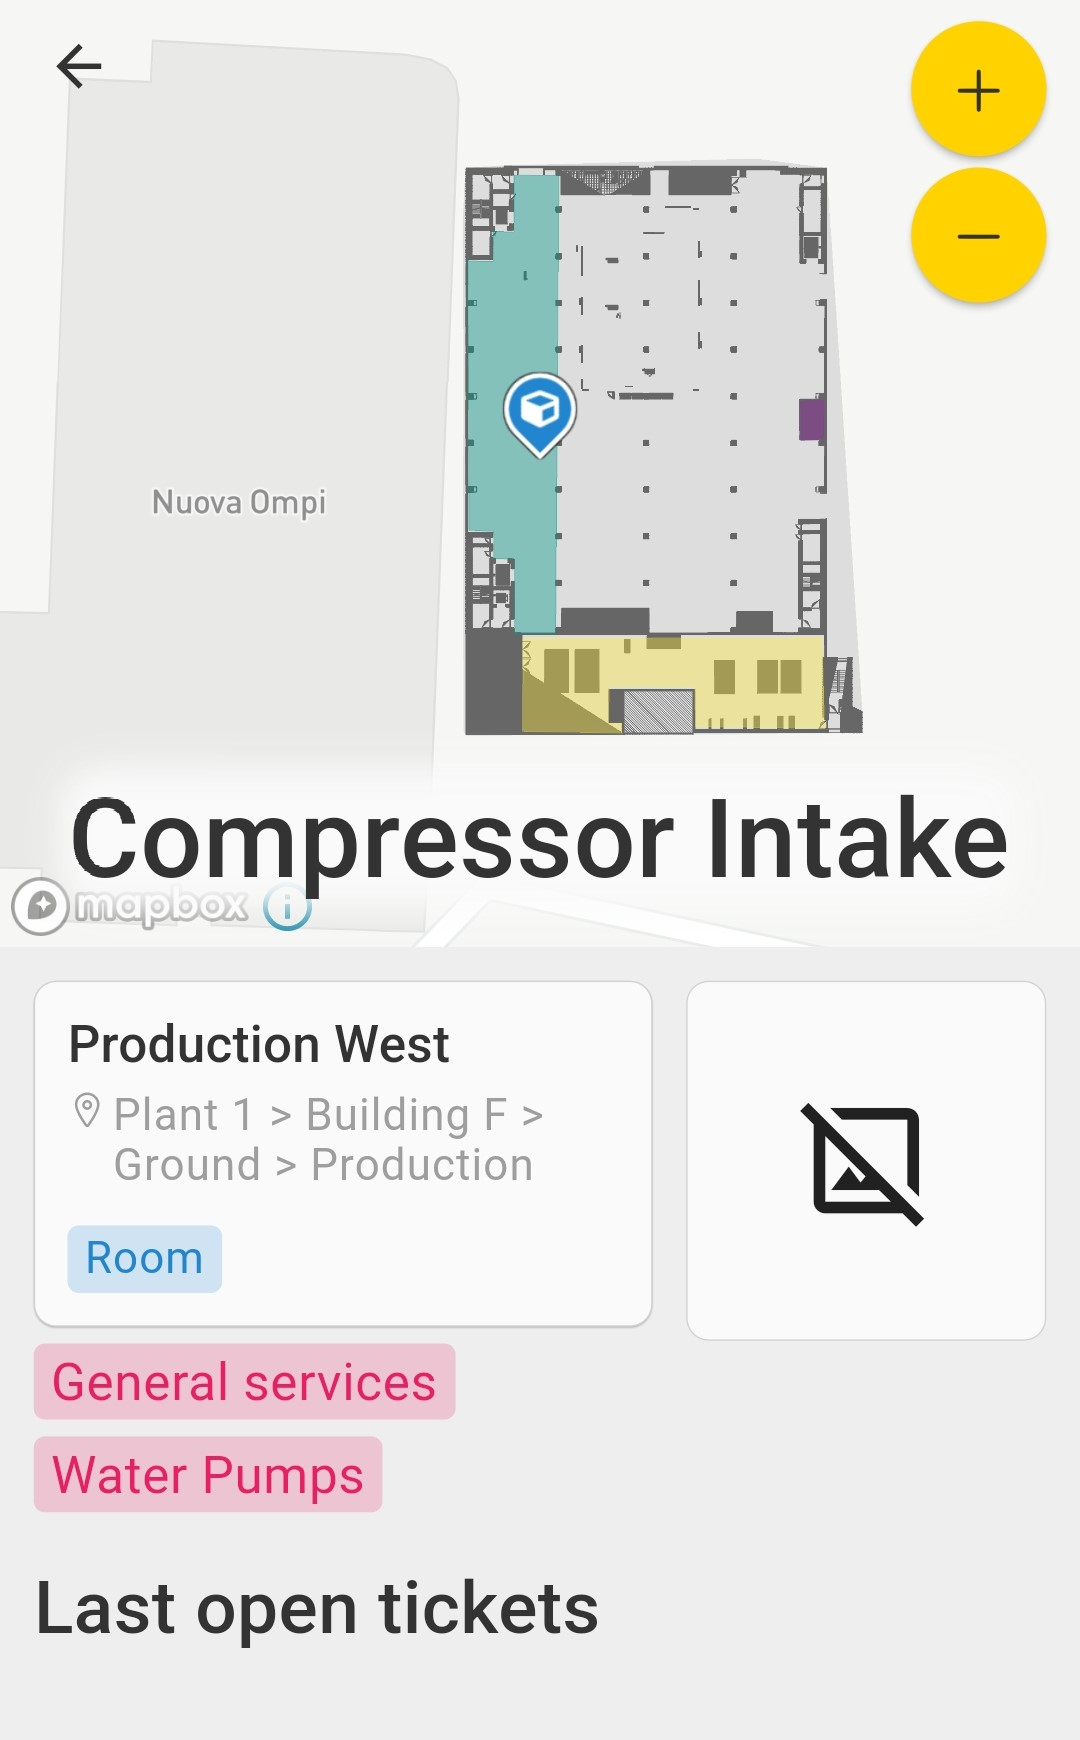
\includegraphics[height=5cm]{plant_asset_screenshot}
    \caption{Asset "Compressor Intake" in stabilimento "Plant 1"}
\end{figure}

Tutte le funzionalità in realtà aumentata dovranno necessariamente appoggiarsi al servizio di \asa{} perchè i gemelli digitali già presenti nel sistema sfruttano proprio questa tecnologia per la propria localizzazione spaziale e, vista la natura multipiattaforma dell'applicazione, dovranno essere implementate sia in Android che in iOS.
Dalla vista dovrà essere possibile interagire con gli \textit{asset} e i \textit{ticket}, (posizionamento ed eliminazione in \textit{augmented reality}) provocando l'apparizione di una \textit{card} all' \textit{on-tap} dell'\textit{anchor}\footnote{Traducibile in italiano con il termine "angoraggio" è un punto di interesse in uno spazio tridimensionale, ovvero un punto che possiede delle coordinate \textit{(x,y,z)}, al quale possono essere collegati \textit{asset}, \textit{ticket} o altri ancoraggi.}, ovvero mostrando a schermo tramite una piccola finestra in sovraimpressione i vari ticket relativi all'\textit{asset} dopo che questo viene toccato, permettendo anche la visione del dettaglio o la rimozione dello stesso.

\begin{figure}[ht]
    \centering
    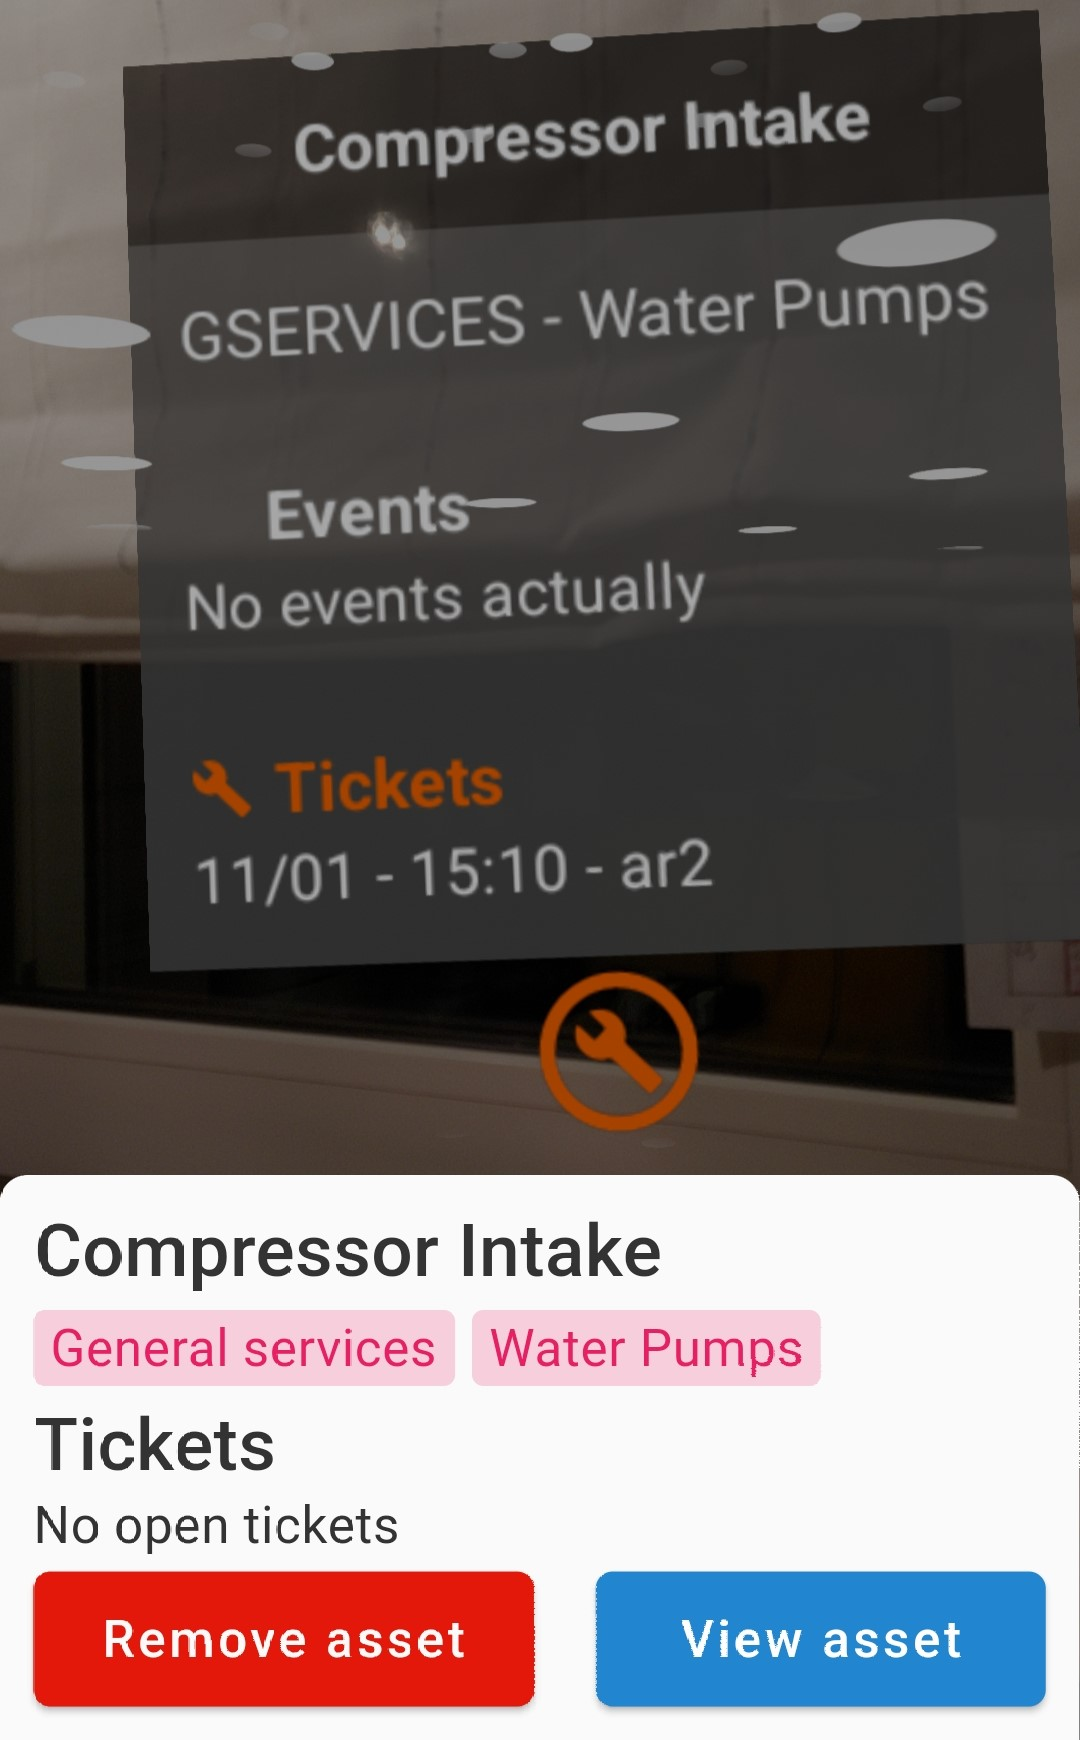
\includegraphics[height=5cm]{asset_card}
    \caption{\textit{Card} (in primo piano) relativa a una \textit{anchor} (in secondo piano) in vista in realtà aumentata}
\end{figure}

Per portare a termine gli obiettivi prefissati sarà necessario studiare dei \textit{framework}, dei \textit{plugin} o dei \sdk{} che permettono l'integrazione del codice nativo di \asa{} (che sarà Java per Android e Swift per iOS) con il \textit{framework} Flutter e il linguaggio su cui si poggia, ovvero Dart. 
\fi
\section{Obiettivi}
\iffalse
\begin{itemize}
    \item Minimi:
        \begin{itemize}
            \item Studio e comprensione del linguaggio di programmazione Dart e del \textit{framework} Flutter;
            \item Analisi strumenti Azure: Azure Console e \asa{};
            \item Ricerca di \textit{framework} e \sdk{} per implementare le \asa{} in Flutter;
            \item Eventuale studio di linguaggi necessari alle implementazioni native, come ad esempio Kotlin, Java, Unity o Swift;
            \item Completamento del \textit{framework} scelto nell'app Flutter esistente;
            \item Completamento dello sviluppo dei componenti per rappresentare le \textit{anchor} nello spazio in realtà aumentata;
            \item Completamento dello sviluppo delle \api{} per l'interazione utente con gli ancoraggi in realtà aumentata;
        \end{itemize}
    \item Massimi: 
        \begin{itemize}
            \item Sviluppo di componenti per mappare \textit{asset} aziendali ad \textit{anchor};
            \item Sviluppo di componenti grafici per la visualizzazione di metriche e informazioni di controllo.
        \end{itemize}
\end{itemize}
\fi
\section{Vincoli}
\iffalse
Come precedentemente accennato, i vincoli in questo progetto sono due: 
\begin{itemize}
    \item Utilizzare Flutter come \textit{framework} sul quale implementare le componenti in realtà aumentata;
    \item La tecnologia scelta per gestire gli ancoraggi in realtà aumentata deve essere \asa{}.
\end{itemize}
Eccezion fatta per queste specifiche tecnologiche il resto è stato lasciato a mia discrezione personale, sebbene siano stati consigliati degli strumenti di sviluppo (\vsc{} e \astudio{} come \ide{}). 
Vincoli non tecnologici ma organizzativi sono da identificare nell'uso di Slack di GitHub: il primo usato per la comnicazione interna con i membri di dell'azienda, il secondo invece è il \textit{repository}\footnote{Spesso abbreviato con \textit{"repo"} è un generico archivio di codice sorgente e pacchetti \textit{software}. Spesso contiene anche \textit{metadata} e guide per la configurazione, uso ed estensione del codice che contiene. In genere un \textit{repo} ha una qualche forma di controllo di versione integrato.} dove si trova il codice sorgente di MobileSYN.
\fi
\section{Motivazione scelta}
\iffalse
I motivi che mi hanno spinto ad accettare questo stage rispetto ad altri sono molteplici, ma i principali sono quattro: toccare con mano attività legate al \textit{frontend}, vivere in prima persona l'ambiente di lavoro del mio ambito di studi, avere la possibilità di sviluppare in ambito \textit{mobile} e una personale curiosità nei confronti delle tecnologie trattate, ovvero la realtà aumentata.
Elaboro ora con più completezza i quattro punti di cui sopra: per quanto riguarda il \textit{frontend}, è un ambito o comunque sia una branca del mondo dello sviluppo \textit{software} che guardavo con interesse in quanto raramente ho avuto occasione di occuparmene durante il corso di studui. Infatti nella maggioranza dei progetti e degli \textit{assignment} trattati mi sono sempre occupato del lato \textit{backend}, infatti il cambio di approccio si è dimostrato difficoltoso, costringendomi a ragionare e a vedere il codice in maniera diversa. Flutter inoltre ha reso il tutto ancora più arduo siccome mischia aspetti di interfaccia grafica con logiche di controllo.\\
Vivere uno stage a contatto con degli sviluppatori di grado \textit{senior} e lavorare in un ambiente con un certo grado di controllo era per me molto importante: da una parte per garantirmi di assorbire conoscenze da personale esperto, dall'altra per assicurarmi di mantenere un \textit{focus} quanto più alto possibile durante il corso del progetto. Era inoltre fondamentale avere un'idea più chiara di come sia il mondo del lavoro in ambito \textit{software}.\\
Il terzo punto nasce da una considerazione: il mondo dello sviluppo \textit{mobile} è quello più ampio e in continua crescita. Ormai i \textit{computer} sono sempre più rari e vengno generalmente acquistati da persone ad alto livello di specializzazione, mentre il pubblico generalista preferisce acquistare \textit{smartphone} e \textit{tablet}. E' quindi saggio a mio avviso sviluppare delle competenze in questo ambito perchè saranno sicuramente molto spendibili.\\
Infine, il quarto ed ultimo motivo che mi ha spinto a scegliere questo \textit{stage} rispetto ad altri riguarda la tecnologia affrontata: trovo affascinante l'impiego della realtà aumentata perchè è molto poco comune e, probabilmente, diventerà man mano più diffusa con il passare degli anni. Inoltre tra quelle disponibili ho trovato intelligente da parte di Datasoil scegliere proprio quella di Microsoft che, forte di disponibilità economiche fuori misura, difficilmente abbandonerà un progetto sul quale ha già investito così largamente.\\
Naturalmente oltre a tutto ciò sono ho avuto un'impressione umana molto positiva durante la riunione di primo contatto avuta con Andrea Ongaro (che poi è diventato il mio tutor aziendale) e Pietro Decaro (amministratore delegato di Datasoil), che mi ha incentivato ad accettare questo specifico progetto.\\
Schematizzo quindi gli obiettivi che voglio perseguire tramite l'esperienza di \textit{stage}:
\begin{itemize}
    \item Acquisire competenze di programmazione \textit{frontend}:
        \begin{itemize}
            \item Utilizzare linguaggi specifici (ad esempio Dart);
            \item Sviluppare componenti grafiche per applicazioni mobile;
            \item Sviluppare familiarità con strumenti comunemente usati (ad esempio \vsc);
        \end{itemize}
    \item Osservare direttamente il lavoro in azienda \textit{software}:
        \begin{itemize}
            \item Vedere organizzazione giornaliera lavori;
            \item Valutare tempistiche e ritmi lavorativi;
            \item Valutare equilibrio vita-lavoro;
        \end{itemize}
    \item Acquisire competenze di sviluppo \textit{mobile}:
        \begin{itemize}
            \item Sviluppare familiarità con strumenti comunemente usati (ad esempio emulatori);
            \item Sviluppare componenti applicazione mobile;
            \item Utilizzare \textit{framework} specifici (ad esempio Flutter);
        \end{itemize}
    \item Acquisire competenze di realtà aumentata:
        \begin{itemize}
            \item Comprendere teoria dietro concetti come ancoraggi e tridimensionalità;
            \item Conoscere tecnologie principali usate nel campo;
            \item Valutare se sia di mio interesse perseguire studi futuri sull'argomento.
        \end{itemize}
\end{itemize}
\fi
